\documentclass[border=10pt]{standalone}
\usepackage{tikz}
\usetikzlibrary{matrix, positioning, arrows.meta, calc}

\definecolor{headerblue}{RGB}{0, 0, 102}
\definecolor{rowgray}{RGB}{240, 240, 240}
\definecolor{totalrow}{RGB}{220, 220, 220}

\tikzset{
    table/.style={
        matrix of nodes,
        row sep=-\pgflinewidth,
        column sep=-\pgflinewidth,
        nodes={rectangle, draw, anchor=center, text width=2.2cm, align=center, minimum height=6mm},
        column 1/.style={nodes={text width=3cm, align=left}},
        row 1/.style={nodes={fill=headerblue, text=white, font=\bfseries}},
        row 2/.style={nodes={fill=rowgray}},
        row 3/.style={nodes={fill=rowgray}},
        row 4/.style={nodes={fill=rowgray}},
        row 5/.style={nodes={fill=rowgray}},
        row 6/.style={nodes={fill=rowgray}},
        row 7/.style={nodes={fill=totalrow}},
        every node/.style={font=\small},
        inner xsep=2pt,
        inner ysep=2pt,
        outer sep=0pt
    },
    header/.style={fill=headerblue, text=white, font=\bfseries},
    data/.style={fill=rowgray},
    total/.style={fill=totalrow},
    border/.style={draw=black, thick},
    headerborder/.style={draw=black, thick, fill=headerblue, text=white, font=\bfseries},
    databorder/.style={draw=black, thick, fill=rowgray},
    totalborder/.style={draw=black, thick, fill=totalrow}
}

\begin{document}
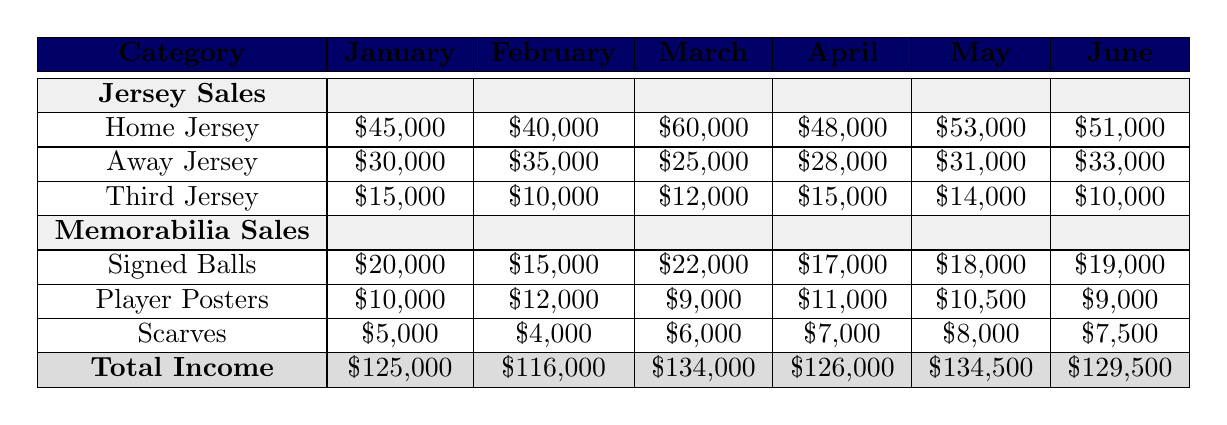
\begin{tikzpicture}
\node (table) {
\begin{tabular}{|c|c|c|c|c|c|c|}
\hline
\rowcolor{headerblue}
\textbf{Category} & \textbf{January} & \textbf{February} & \textbf{March} & \textbf{April} & \textbf{May} & \textbf{June} \\
\hline
\hline
\rowcolor{rowgray}
\textbf{Jersey Sales} & & & & & & \\
\hline
Home Jersey & \$45,000 & \$40,000 & \$60,000 & \$48,000 & \$53,000 & \$51,000 \\
\hline
Away Jersey & \$30,000 & \$35,000 & \$25,000 & \$28,000 & \$31,000 & \$33,000 \\
\hline
Third Jersey & \$15,000 & \$10,000 & \$12,000 & \$15,000 & \$14,000 & \$10,000 \\
\hline
\rowcolor{rowgray}
\textbf{Memorabilia Sales} & & & & & & \\
\hline
Signed Balls & \$20,000 & \$15,000 & \$22,000 & \$17,000 & \$18,000 & \$19,000 \\
\hline
Player Posters & \$10,000 & \$12,000 & \$9,000 & \$11,000 & \$10,500 & \$9,000 \\
\hline
Scarves & \$5,000 & \$4,000 & \$6,000 & \$7,000 & \$8,000 & \$7,500 \\
\hline
\rowcolor{totalrow}
\textbf{Total Income} & \$125,000 & \$116,000 & \$134,000 & \$126,000 & \$134,500 & \$129,500 \\
\hline
\end{tabular}
};
\end{tikzpicture}
\end{document}